
%!TEX root = ./main.tex



\tikzset{every picture/.style={line width=0.75pt}} %set default line width to 0.75pt        

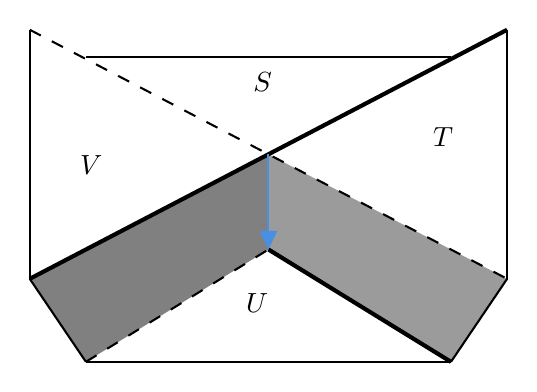
\begin{tikzpicture}[x=0.75pt,y=0.75pt,yscale=-1,xscale=1]
%uncomment if require: \path (0,877); %set diagram left start at 0, and has height of 877

%Straight Lines [id:da6932355685480536] 
\draw [draw opacity=0][fill={rgb, 255:red, 155; green, 155; blue, 155 }  ,fill opacity=1 ]   (412.94,200) -- (440,160) -- (325,100) -- (325,145.87) -- cycle ;
%Straight Lines [id:da1384787451044316] 
\draw [draw opacity=0][fill={rgb, 255:red, 128; green, 128; blue, 128 }  ,fill opacity=1 ]   (210,160) -- (237.06,200) -- (315.46,151.74) -- (325,145.87) -- (325,100) -- cycle ;
%Straight Lines [id:da0741744233702265] 
\draw [line width=1.5]    (210,160) -- (440,40) ;
%Straight Lines [id:da5955578937587962] 
\draw  [dash pattern={on 4.5pt off 4.5pt}]  (210,40) -- (440,160) ;
%Straight Lines [id:da85493541645859] 
\draw    (210,160) -- (237.06,200) ;
%Straight Lines [id:da7842887989072671] 
\draw    (440,160) -- (412.94,200) ;
%Straight Lines [id:da2669884694205853] 
\draw    (210,40) -- (210,160) ;
%Straight Lines [id:da637854901562851] 
\draw    (440,40) -- (440,160) ;
%Straight Lines [id:da7206676036750514] 
\draw [color={rgb, 255:red, 74; green, 144; blue, 226 }  ,draw opacity=1 ]   (325,100) -- (325,142.87) ;
\draw [shift={(325,145.87)}, rotate = 270] [fill={rgb, 255:red, 74; green, 144; blue, 226 }  ,fill opacity=1 ][line width=0.08]  [draw opacity=0] (8.93,-4.29) -- (0,0) -- (8.93,4.29) -- cycle    ;
%Straight Lines [id:da12493325383084064] 
\draw [line width=1.5]    (325,145.87) -- (412.94,200) ;
%Straight Lines [id:da0009226395893477957] 
\draw  [dash pattern={on 4.5pt off 4.5pt}]  (237.06,200) -- (325,145.87) ;
%Straight Lines [id:da06537491608635204] 
\draw    (237.06,200) -- (412.94,200) ;
%Straight Lines [id:da9541213893361323] 
\draw    (237.06,53.33) -- (412.94,53.33) ;

% Text Node
\draw (316.29,59.07) node [anchor=north west][inner sep=0.75pt]    {$S$};
% Text Node
\draw (232.76,99.07) node [anchor=north west][inner sep=0.75pt]    {$V$};
% Text Node
\draw (402.88,85.73) node [anchor=north west][inner sep=0.75pt]    {$T$};
% Text Node
\draw (312.76,165.73) node [anchor=north west][inner sep=0.75pt]    {$U$};


\end{tikzpicture}